\documentclass{standalone}

\usepackage{tikz}
\usepackage[T1]{fontenc}
\usepackage[tt=false, type1=true]{libertine}
\usepackage[varqu]{zi4}
\usepackage[libertine]{newtxmath}

\usetikzlibrary{shapes, positioning, calc}

\begin{document}

{\scriptsize
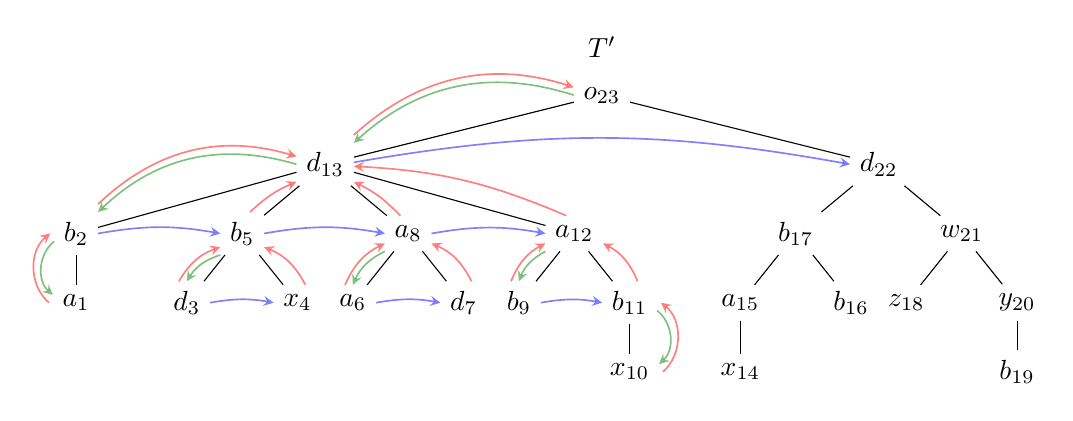
\begin{tikzpicture}[
    level distance=2.5em,
    level 1/.style={sibling distance=20em},
    level 2/.style={sibling distance=6em},
    level 3/.style={sibling distance=4em},
    level 4/.style={sibling distance=2em}]

  \tikzset{ptr/.style={semithick, ->, >=stealth, opacity=0.5}}
  \tikzset{parptr/.style={ptr, red}}
  \tikzset{c1ptr/.style={ptr, black!50!green}}
  \tikzset{sibptr/.style={ptr, blue}}

  % document
  \node at (0, 0) (o23) {$o_{23}$}
  child {
    node (d13) {$d_{13}$}
    child {
      node (b2) {$b_2$}
      child { node (a1) {$a_1$} }
    }
    child {
      node (b5) {$b_5$}
      child { node (d3) {$d_3$} }
      child { node (x4) {$x_4$} }
    }
    child {
      node (a8) {$a_8$}
      child { node (a6) {$a_6$} }
      child { node (d7) {$d_7$} }
    }
    child {
      node (a12) {$a_{12}$}
      child { node (b9) {$b_9$} }
      child {
        node (b11) {$b_{11}$}
        child { node (x10) {$x_{10}$} }
      }
    }
  }
  child {
    node (d22) {$d_{22}$}
    child {
      node (b17){$b_{17}$}
      child {
        node (a15) {$a_{15}$}
        child { node (x14) {$x_{14}$} }
      }
      child { node (b16) {$b_{16}$} }
    }
    child {
      node (w21) {$w_{21}$}
      child { node (z18) {$z_{18}$} }
      child {
        node (y20) {$y_{20}$}
        child { node (b19) {$b_{19}$} }
      }
    }
  };
  \node[above=0.125 of o23] (t1) {$T'$};

  % parent pointers
  \draw[parptr] ($(d13.north east)+(0, 0.1)$) to[bend left] ($(o23.west)+(0, 0.1)$);
  \draw[parptr] ($(b2.north east)+(0, 0.1)$) to[bend left] ($(d13.west)+(0, 0.1)$);
  \draw[parptr] ($(a1.west)+(-0.05, 0)$) to[bend left=50] ($(b2.west)+(-0.05, 0)$);
  \draw[parptr] ($(b5.north)+(0.1, 0)$) to[bend left=10] ($(d13.south west)+(0, 0.05)$);
  \draw[parptr] ($(d3.north)+(-0.1, 0)$) to[bend left=20] ($(b5.south west)+(0, 0.1)$);
  \draw[parptr] ($(x4.north)+(0.1, 0)$) to[bend right=20] ($(b5.south east)+(0, 0.1)$);
  \draw[parptr] ($(a8.north)+(-0.1, 0)$) to[bend right=10] ($(d13.south east)+(0, 0.05)$);
  \draw[parptr] ($(a6.north)+(-0.1, 0)$) to[bend left=20] ($(a8.south west)+(0, 0.1)$);
  \draw[parptr] ($(d7.north)+(0.1, 0)$) to[bend right=20] ($(a8.south east)+(0, 0.1)$);
  \draw[parptr] ($(a12.north)+(-0.1, 0)$) to[bend right=10] ($(d13.east)+(0, -0.025)$);
  \draw[parptr] ($(b9.north)+(-0.1, 0)$) to[bend left=20] ($(a12.south west)+(0, 0.1)$);
  \draw[parptr] ($(b11.north)+(0.1, 0)$) to[bend right=20] ($(a12.south east)+(0, 0.1)$);
  \draw[parptr] ($(x10.east)+(0.05, 0)$) to[bend right=50] ($(b11.east)+(0.05, 0)$);

  % first child pointers
  \draw[c1ptr] (o23.west) to[bend right] (d13.north east);
  \draw[c1ptr] (d13.west) to[bend right] (b2.north east);
  \draw[c1ptr] ($(b2.west)+(0, -0.1)$) to[bend right=50] ($(a1.west)+(0, 0.1)$);
  \draw[c1ptr] (b5.south west) to[bend right=20] (d3.north);
  \draw[c1ptr] (a8.south west) to[bend right=20] (a6.north);
  \draw[c1ptr] (a12.south west) to[bend right=20] (b9.north);
  \draw[c1ptr] ($(b11.east)+(0, -0.1)$) to[bend left=50] ($(x10.east)+(0, 0.1)$);

  % nex (right) sibling pointers
  \draw[sibptr] ($(d13.east)+(0, 0.025)$) to[bend left=10] (d22.west);
  \draw[sibptr] (b2.east) to[bend left=10] (b5.west);
  \draw[sibptr] (b5.east) to[bend left=10] (a8.west);
  \draw[sibptr] (a8.east) to[bend left=10] (a12.west);
  \draw[sibptr] (d3.east) to[bend left=10] (x4.west);
  \draw[sibptr] (a6.east) to[bend left=10] (d7.west);
  \draw[sibptr] (b9.east) to[bend left=10] (b11.west);
\end{tikzpicture}}

\end{document}
